%----------------------------------------------------------------------------------------
%    PACKAGES AND OTHER DOCUMENT CONFIGURATIONS
%----------------------------------------------------------------------------------------

\documentclass[a4paper,10pt]{memoir} % Font and paper size


%----------------------------------------------------------------------------------------
%	PACKAGES AND OTHER DOCUMENT CONFIGURATIONS
%----------------------------------------------------------------------------------------
\usepackage[top=1cm,left=1cm,right=1cm,bottom=1cm]{geometry} % Modify margins
\usepackage{XCharter} % Use the Bitstream Charter font
\usepackage[utf8]{inputenc} % Required for inputting international characters
\usepackage[T1]{fontenc} % Output font encoding for international characters

\usepackage{graphicx} % Required for figures

\usepackage{flowfram} % Required for the multi-column layout

\usepackage{url} % URLs

\usepackage[usenames,dvipsnames]{xcolor} % Required for custom colours

\usepackage{tikz} % Required for the horizontal rule

\usepackage{enumitem} % Required for modifying lists
\setlist{noitemsep,nolistsep} % Remove spacing within and around lists    noitemsep,nolistsep

\setlength{\columnsep}{\baselineskip} % Set the spacing between columns

% Define the left frame (sidebar)
\newflowframe{0.23\textwidth}{\textheight}{0pt}{0pt}[left]
\newlength{\LeftMainSep}
\setlength{\LeftMainSep}{0.22\textwidth} %left space of border
\addtolength{\LeftMainSep}{1\columnsep}
 
% Small static frame for the vertical line
\newstaticframe{1.5pt}{\textheight}{\LeftMainSep}{0pt}
 
% Content of the static frame with the vertical line
\begin{staticcontents}{1}
\hfill
\tikz{\draw[loosely dotted,color=RoyalBlue,line width=1.5pt,yshift=0](0,0) -- (0,\textheight);}
\hfill\mbox{}
\end{staticcontents}
 
% Define the right frame (main body)
\addtolength{\LeftMainSep}{1.5pt}
\addtolength{\LeftMainSep}{1\columnsep}
\newflowframe{0.7\textwidth}{\textheight}{\LeftMainSep}{0pt}[main01]

\pagestyle{empty} % Disable all page numbering

\setlength{\parindent}{0pt} % Stop paragraph indentation

%----------------------------------------------------------------------------------------
%	NEW COMMANDS
%----------------------------------------------------------------------------------------

\newcommand{\userinformation}[1]{\renewcommand{\userinformation}{#1}} % Define a new command for the CV user's information that goes into the left column

\newcommand{\cvheading}[1]{{\Huge\bfseries\color{RoyalBlue} #1} \par\vspace{.6\baselineskip}} % New command for the CV heading
\newcommand{\cvsubheading}[1]{{\Large\bfseries #1} \bigbreak} % New command for the CV subheading

\newcommand{\Sep}{\vspace{1em}} % New command for the spacing between headings
\newcommand{\SmallSep}{\vspace{0.5em}} % New command for the spacing within headings

\newcommand{\aboutme}[2]{ % New command for the about me section
\textbf{\color{RoyalBlue} #1}~~#2\par\Sep
}
	
\newcommand{\CVSection}[1]{ % New command for the headings within sections
{\Large\textbf{#1}}\par
\SmallSep % Used for spacing
}

\newcommand{\CVItem}[2]{ % New command for the item descriptions
\textbf{\color{RoyalBlue} #1}\par
#2
\SmallSep % Used for spacing
}

\newcommand{\cvsubitem}[1]{ % New command for the item descriptions
\textbf{\color{RoyalBlue} #1}
}

\newcommand{\cvpub}[4]{ % New command for the item descriptions
#1 (#2) : \textbf{"#3"}, \textit{#4} 
% \textbf{\color{RoyalBlue} #1}
}

\newcommand{\bluebullet}{\textcolor{RoyalBlue}{$\circ$}~~} % New command for the blue bullets
 % Include the file specifying document layout and packages


\userinformation{ % Set the content that goes into the sidebar of each page
\begin{flushright}

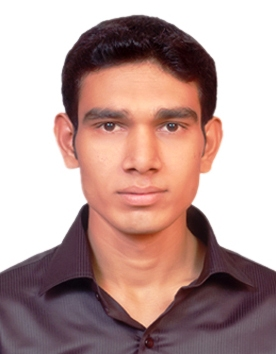
\includegraphics[width=.6\columnwidth]{photo.jpg}\\[\baselineskip] % Your photo
\small % Smaller font size
\textbf{Nikhil M. Dhandre} \\ % Your name
\url{nik.digitronik@live.com} \\ % Your email address
\url{www.digitronik.in} \\ % Your URL
\url{www.github.com/digitronik}\\ % Your git
\texttt{+91-9096919955} \\ % Your phone number
\Sep % Some whitespace
\textbf{Date of Birth} \\
\texttt{April 04, 1991}\\

% \Sep % Some whitespace
% \textbf{Address} \\
% 3642, Shastri Nagar, \\ % Address 1
% Near Dr. Ambedkar School, \\ % Address 2
% Armori, \\ % Address 3
% MH-441208.\\

\Sep % Some whitespace
\textbf{Address} \\
\texttt{B-1001, Sarang, \\ % Address 1
Nanded City, \\ % Address 2
Pune, \\ % Address 3
MH-411041.}
\vfill % Whitespace under this block to push it up under the photo
\end{flushright}
}




%----------------------------------------------------------------------------------------
%    Start Resume building
%----------------------------------------------------------------------------------------

\begin{document}

\userinformation % Print your information in the left column
\framebreak % End of the first column

%----------------------------------------------------------------------------------------
%    HEADING
%----------------------------------------------------------------------------------------

\cvheading{\textsc{Nikhil Dhandre}} % Large heading - your name

% \cvsubheading{Software Engineer} % Subheading - your occupation/specialization
\Sep
%----------------------------------------------------------------------------------------
%    ABOUT ME
%----------------------------------------------------------------------------------------
% \aboutme{About Me:}{A result-oriented Engineer with one year seven month of experience in the area of Research and Software. 
% Seeking for challenging and creative environment in order to utilise my technical knowledge, educational background for effectively
% contribute to the growth of the organisation.}
\aboutme{About Me:}{
A result-oriented Engineer with one year seven month of experience in the area of Research and Quality Engineering.
Seeking for challenging and creative environment in order to utilise my technical knowledge, educational background for effectively
contribute to the growth of the organisation.}

\Sep % Extra whitespace after the end of a major section
%----------------------------------------------------------------------------------------
%    SKILLS
%----------------------------------------------------------------------------------------

\CVSection{\textsc{Skill Set}:}

%------------------------------------------------
\begin{minipage}[t]{0.20\columnwidth}
\cvsubitem{Languages} \\
\cvsubitem{Frameworks} \\
\cvsubitem{Databases} \\
\cvsubitem{Servers} \\
\cvsubitem{OS}\\
\cvsubitem{Softwares} \\
\quad \\
\cvsubitem{Hardware}\\
\cvsubitem{Courses}

\end{minipage}
\hfill
\begin{minipage}[t]{0.80\columnwidth}
: Python, C, Shell, \LaTeX, HTML, PL/SQL, PHP (\textit{basic})\\
: Pytest, Navmazing, Widgetastic, Wrapanapi\\ 
: MySQL, PostgreSQL, SQLite \\ 
: LAMP (\textit{Apache}), FTP, Mailing \\
: Linux, Windows\\
: Proteus, Multisim, Matlab, Keil, Arduino, Kile,\\ \phantom{.} %blank space
Express PCB, Photoshop, Altium (\textit{just start}) etc.\\
: Raspberry Pi, Arduino, Microcontrollers\\ 
: CCO, CCC
\end{minipage}
% {\begin{tabular}{p{0.2\textwidth} p{0.2\textwidth} p{0.2\textwidth}}
% \bluebullet Java &  \bluebullet Shell & \bluebullet Python\\
% \bluebullet C++ &  \bluebullet PHP & \bluebullet Matlab\\
% \end{tabular}}
% \vspace{.2cm}

%----------------------------------------------------------------------------------------
%    Organisational Scan

% RedHat 20 Dec 2017
% IMD 20 Apr 2016 - 19 Jun 2017 > 1yr 2 month
%----------------------------------------------------------------------------------------
\Sep % Extra whitespace after the end of a major section
\Sep
\CVSection{\textsc{Organisational Scan}:}

\begin{minipage}[t]{0.20\columnwidth}
\cvsubitem{Since Jun'20}
\end{minipage}
\hfill
\begin{minipage}[t]{0.80\columnwidth}
\begin{center}
\cvsubitem{Red Hat India Pvt.Ltd, Pune}\\
\textbf{(Intern)}
\end{center}
\end{minipage}
\Sep

\begin{minipage}[t]{0.20\columnwidth}
\textbf{Team}\\
\textbf{Technologies}\\
\textbf{Role}\\
\textbf{Repository}\\
\textbf{Description}
\end{minipage}
\hfill
\begin{minipage}[t]{0.80\columnwidth}
: \textbf{\textsc{Cloud Forms Management Engine (CFME) QE}}\\
: Python, Pytest, Widgetastic, Navmazing, Wrapanapi\\
: I am responsible for Quality Engineering.\\
: \url{https://github.com/ManageIQ/integration_tests}\\
: \begin{itemize}
\renewcommand{\labelitemi}{\bluebullet}
\item Responsible for focus areas(Storage, Provider Discovery, Capacity, and Utilization) 
\item Added Model pages for Storage in the framework
\item Automate new test cases as well as fixed broken automation 
\item Contributed in core Widgetastic framework 
\item Enhanced the test coverage for Capacity and Utilization
\item Maintain Polarion test cases
\item Added Mojo Page for cfme storage feature 
  \end{itemize}

\end{minipage}

\Sep
\Sep
\begin{minipage}[t]{0.20\columnwidth}
\cvsubitem{Apr'16-Jun'17}
\end{minipage}
\hfill
\begin{minipage}[t]{0.80\columnwidth}
\begin{center}
\cvsubitem{India Meteorological Department (IMD), Pune}\\
\textbf{(Junior Research Fellow)}  
\end{center}
\end{minipage}

\Sep
\begin{minipage}[t]{0.20\columnwidth}
% synop decoder
\textbf{(Project-1)}\\
\textbf{Technologies}\\
\textbf{Role}\\
\textbf{Repository}\\
\textbf{Description}

\vspace{13mm}

% MAWS
\textbf{(Project-2)}\\
\textbf{Technologies}\\
\textbf{Role}\\
\textbf{Description}

\vspace{8.1 mm}

% GRIB2Reader
\textbf{(Project-3)}\\
\textbf{Technologies}\\
\textbf{Role}\\
\textbf{Repository}\\
\textbf{Description}\\

\end{minipage}
\hfill
\begin{minipage}[t]{0.80\columnwidth}
: \textbf{\textsc{SYNOP Decoder}}\\
: Python, MySQL\\
: I was responsible for development.\\
: \url{https://github.com/digitronik/synop-decoder}\\
: This decoder is decoding the Meteorological Global Telecommunication System (GTS) 
Messages (in WMO standard) received from RTH server Pune to National Data Center (NDC) 80 bit Indian standard. \\

: \textbf{\textsc{Mini Automatic Weather Station} (MAWS)}\\
: Python, MySQL, Embedded, Web Server \\
: I was responsible for Codding \& Designing.\\
: It is low-cost weather station for increasing the meteorological data traffic. 
It has a Data Logger and Remote monitoring system.\\

: \textbf{\textsc{GRIB Reader}}\\
: Python (\textit{pygrib, matplotlib, pygrib})\\
: I was responsible for development.\\
: \url{https://github.com/digitronik/grib}\\
: GRIB Reader is the utility to read that GRIdded Binary (GRIB) data with respect to Lat-Lon and plotting, export in CSV, compares data, point value.\\
\end{minipage}


%----------------------------------------------------------------------------------------
%    NEW PAGE DELIMITER
%    Place this block wherever you would like the content of your CV to go onto the next page
%----------------------------------------------------------------------------------------

\clearpage % Start a new page
% \phantom{This text will be invisible}
\userinformation % Print your information in the left column
\framebreak % End of the first column

\begin{minipage}[t]{0.20\columnwidth}
\textbf{(Project-4)}\\
\textbf{Technologies}\\
\textbf{Role}\\
\textbf{Description}\\
\end{minipage}
\begin{minipage}[t]{0.80\columnwidth}
: \textbf{\textsc{AMO Mailing Client}}\\
: Python, SMTP\\
: I was responsible for development.\\
: It is supporting in centralising Drishti System data from various Airports runways in India.
\end{minipage}


\Sep
\Sep
\begin{minipage}[t]{0.20\columnwidth}
\cvsubitem{Agu'15-Jul'16}
\end{minipage}
\hfill
\begin{minipage}[t]{0.80\columnwidth}
\begin{center}
\cvsubitem{Central Water and Power Research Station, Pune}\\
\textbf{(Project Student)}
\end{center}
\end{minipage}
\Sep

\begin{minipage}[t]{0.20\columnwidth}
\textbf{(Project)}\\
\textbf{Technologies}\\
\textbf{Role}\\
\textbf{Description}
\end{minipage}
\hfill
\begin{minipage}[t]{0.80\columnwidth}
: \textbf{\textsc{Dam \& Weather Parameters Monitoring System}}\\
: IoT, Python, MySQL, Webserver\\
: I was responsible for development.\\
: Dam authority facing problems like Manual data observation and transmission results in a considerable time lag between data observed in the field and decision making level so there may be a possibility of losing a real-time data. 
This proposed scheme is used to solve those problems.
\end{minipage}


%----------------------------------------------------------------------------------------
%    Other Experince
%----------------------------------------------------------------------------------------
\Sep % Extra whitespace after the end of a major section
\Sep
\CVSection{\textsc{Other Contributions}:}
\begin{minipage}[t]{0.15\columnwidth}
\textbf{Oct 2017}\\
\\
\textbf{Feb 2016}\\
\\
\textbf{Jul 2015} 
\end{minipage}
\hfill
\begin{minipage}[t]{0.85\columnwidth}
Contribute to Python Workshop under banner of Python Express conducted at RIT, Islampur, Sangli.\\
Resource person for Research Methodology (\LaTeX) Workshop in 
Sinhgad Institue of Technology \& Science, Pune.\\
Conducted a workshop on \LaTeX \, at NPCOE, Gadchiroli.
\end{minipage}





%----------------------------------------------------------------------------------------
%    Publications
%----------------------------------------------------------------------------------------
\Sep % Extra whitespace after the end of a major section
\Sep
\CVSection{\textsc{Publications}:}

\begin{itemize}
 \renewcommand{\labelitemi}{\bluebullet}
 \item \cvpub{Nikhil M. Dhandre, JKS Yadav, Dr. G. Krishnakumar}{Dec-2016}{Design \& Implementation of Mini Automatic Weather Station for
Rural Areas in India}{National Symposium on Tropical Meteorology(TROPMET-2016)}, In Progress.
\SmallSep
 \item \cvpub{Nikhil M. Dhandre, P. D. Kamalasekaran}{Oct-2016}{Dam Parameters Monitoring System}{$7^{th}$IEEE India International Conference on Power Electronics},DOI: 10.1109/IICPE.2016.8079375.
\SmallSep 
 \item \cvpub{Nikhil M. Dhandre, M. M. Jadhav}{Jun-2016}{Dam Data Collection \& Monitoring System}{International Journal of Science and Research}, Vol.5, Issue 6, pp.1787-1790.
\end{itemize}


%----------------------------------------------------------------------------------------
%    ACADEMIC CREDENTIALS
%----------------------------------------------------------------------------------------
\Sep % Extra whitespace after the end of a major section
\CVSection{\textsc{Academic Credentials}:}
\begin{minipage}[t]{0.05\columnwidth}
\textbf{2016}\\
\\
\textbf{2013}\\
\textbf{2012}\\
\\
\textbf{2008}\\ 
\\
\textbf{2006}
\end{minipage}
\hfill
\begin{minipage}[t]{0.90\columnwidth}
\textbf{M.E.} (\texttt{Communication Network}) from Pune University. Secured 8.33 CGPA with Distinction.\\
\textbf{GATE} Qualified.\\
\textbf{B.E.} (\texttt{Electronics Communication}) from Nagpur University. Secured 65.45 with First class.\\
\textbf{H.S.C} (\texttt{Electronics}) from Maharashtra State Board. Secured 73.83\% with First class.\\
\textbf{S.S.C} from Maharashtra State Board. Secured 76.80\% with Distinction.
\end{minipage} \\


%----------------------------------------------------------------------------------------
%    Declaration
%----------------------------------------------------------------------------------------

\vspace{1cm}
I hereby declare that all the information given in my resume is true to the best of my knowledge.
\vspace{1cm}
\begin{flushleft}
\textbf{\small Date} \hspace{0.20cm}:\, \\
\textbf{\small Place}\hspace{0.21cm}:\,    
\end{flushleft}

\begin{flushright}
\textbf{(\small Nikhil M. Dhandre)} 
\end{flushright}

\end{document}
